% Created 2021-09-12 Sun 22:49
% Intended LaTeX compiler: xelatex
\documentclass[letterpaper]{article}
\usepackage{graphicx}
\usepackage{grffile}
\usepackage{longtable}
\usepackage{wrapfig}
\usepackage{rotating}
\usepackage[normalem]{ulem}
\usepackage{amsmath}
\usepackage{textcomp}
\usepackage{amssymb}
\usepackage{capt-of}
\usepackage{hyperref}
\usepackage[margin=1in]{geometry}
\usepackage{fontspec}
\usepackage{indentfirst}
\setmainfont[ItalicFont = LiberationSans-Italic, BoldFont = LiberationSans-Bold, BoldItalicFont = LiberationSans-BoldItalic]{LiberationSans}
\newfontfamily\NHLight[ItalicFont = LiberationSansNarrow-Italic, BoldFont       = LiberationSansNarrow-Bold, BoldItalicFont = LiberationSansNarrow-BoldItalic]{LiberationSansNarrow}
\newcommand\textrmlf[1]{{\NHLight#1}}
\newcommand\textitlf[1]{{\NHLight\itshape#1}}
\let\textbflf\textrm
\newcommand\textulf[1]{{\NHLight\bfseries#1}}
\newcommand\textuitlf[1]{{\NHLight\bfseries\itshape#1}}
\usepackage{fancyhdr}
\pagestyle{fancy}
\usepackage{titlesec}
\usepackage{titling}
\makeatletter
\lhead{\textbf{\@title}}
\makeatother
\rhead{\textrmlf{Compiled} \today}
\lfoot{\theauthor\ \textbullet \ \textbf{2021-2022}}
\cfoot{}
\rfoot{\textrmlf{Page} \thepage}
\titleformat{\section} {\Large} {\textrmlf{\thesection} {|}} {0.3em} {\textbf}
\titleformat{\subsection} {\large} {\textrmlf{\thesubsection} {|}} {0.2em} {\textbf}
\titleformat{\subsubsection} {\large} {\textrmlf{\thesubsubsection} {|}} {0.1em} {\textbf}
\setlength{\parskip}{0.45em}
\renewcommand\maketitle{}
\author{Houjun Liu}
\date{\today}
\title{Day 1 with Alexa --- Jack}
\hypersetup{
 pdfauthor={Houjun Liu},
 pdftitle={Day 1 with Alexa --- Jack},
 pdfkeywords={},
 pdfsubject={},
 pdfcreator={Emacs 28.0.50 (Org mode 9.4.4)}, 
 pdflang={English}}
\begin{document}

\maketitle


\section{Landscapes of Self and Other}
\label{sec:org0c49c01}
\emph{"Nice and Broad and Vague"}

\begin{itemize}
\item The journey of "self"
\item How we other people
\end{itemize}

\subsection{Essential Questions of English 10}
\label{sec:org25b37d0}
\begin{figure}[htbp]
\centering
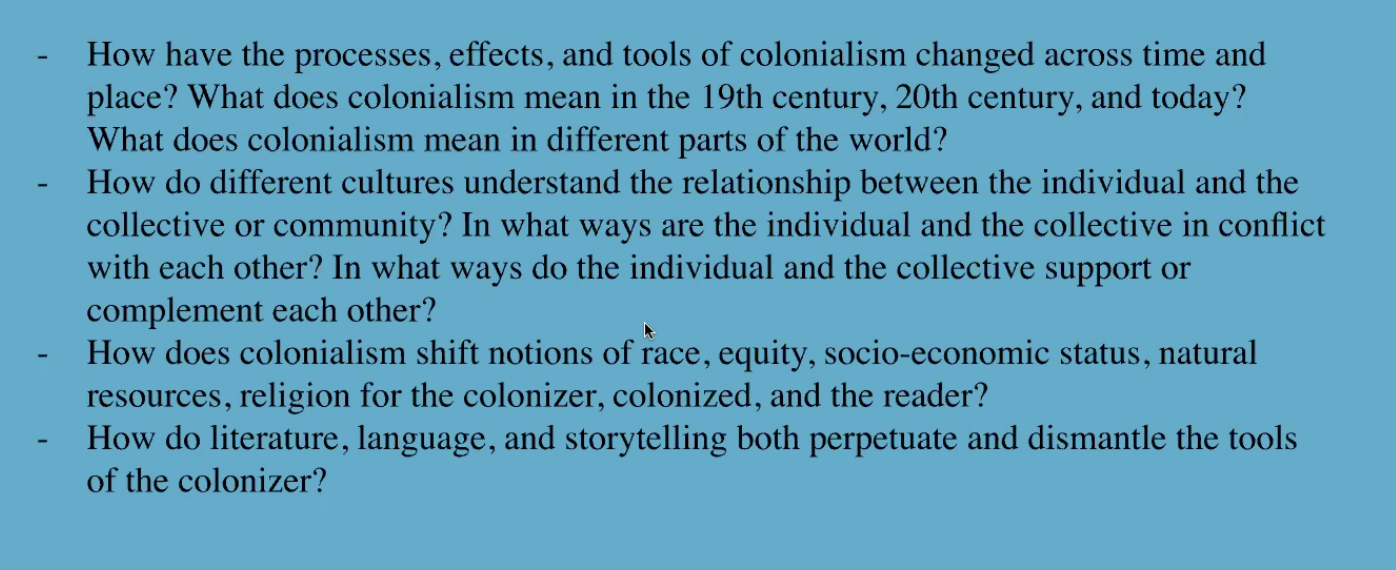
\includegraphics[width=.9\linewidth]{./Screen Shot 2020-08-25 at 1.29.30 PM.png}
\caption{Screen Shot 2020-08-25 at 1.29.30 PM.png}
\end{figure}

And now, an \textbf{assignment} to begin the year:

\section{Four Questions}
\label{sec:org40f9f51}
\begin{itemize}
\item What do you love learning about?
\end{itemize}

I love learning about all facets of human experience. However, I have a
particular interest about computer science + ethics and how it connects
to philosophy.

\begin{itemize}
\item What are you most looking forward to this school year?
\end{itemize}

I look forward to being back in class --- working with everyone in
person and being able to have organic and captivating conversations
spontaneously.

\begin{itemize}
\item What is a favorite book or film?
\end{itemize}

My favourite book is probably, at the moment, Triggers by Marshall
Goldsmith.

I don't actually watch a lot of movies ;)

\begin{itemize}
\item What you want to work on in English class this semester?
\end{itemize}

For this year in English, I look forward to performing more holistic
analysis of texts: tracking items not just on the micro level (word
choice, motifs, etc.) nor just on the macro level (plot, theme) but
being able to effectively connect them together.

\section{Think-Pair-Share}
\label{sec:orge471f50}
\emph{These are our answers, not definitive}

See
\href{KBhENG201TPSGlobalizationColonialismImperialism.org}{KBhENG201TPSGlobalizationColonialismImperialism}
ThinkPairShare --- Globalization, Colonization, Imperialism.

\section{And now, surrealism}
\label{sec:orga68f09f}
Homework: Read! \emph{The I is Never Alone}.
\href{KBhENG201TheIIsNeverAlone.org}{KBhENG201TheIIsNeverAlone}
\end{document}
